

\tikzset{every picture/.style={line width=0.75pt}} %set default line width to 0.75pt        

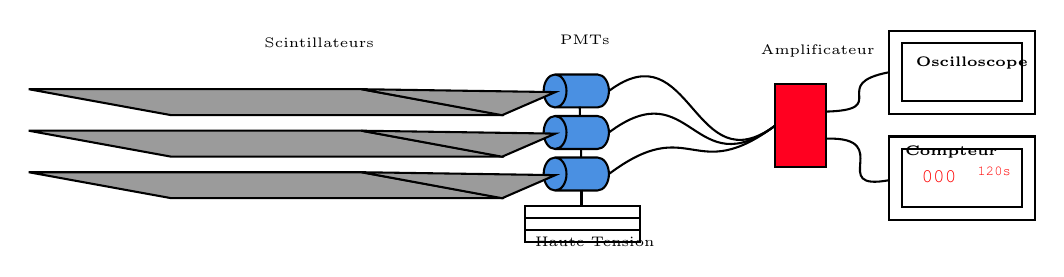
\begin{tikzpicture}[x=0.75pt,y=0.75pt,yscale=-1,xscale=1]
%uncomment if require: \path (0,300); %set diagram left start at 0, and has height of 300

%Shape: Parallelogram [id:dp35301618885454245] 
\draw  [fill={rgb, 255:red, 155; green, 155; blue, 155 }  ,fill opacity=1 ][line width=0.75]  (234.63,54.2) -- (74.3,54.2) -- (143.01,66.72) -- (303.34,66.72) -- cycle ;
%Flowchart: Direct Access Storage [id:dp1191186204993182] 
\draw  [fill={rgb, 255:red, 74; green, 144; blue, 226 }  ,fill opacity=1 ][line width=0.75]  (327.9,63) -- (348.34,63) .. controls (351.38,63) and (353.84,59.45) .. (353.84,55.06) .. controls (353.84,50.67) and (351.38,47.12) .. (348.34,47.12) -- (327.9,47.12)(322.4,55.06) .. controls (322.4,59.45) and (324.86,63) .. (327.9,63) .. controls (330.94,63) and (333.4,59.45) .. (333.4,55.06) .. controls (333.4,50.67) and (330.94,47.12) .. (327.9,47.12) .. controls (324.86,47.12) and (322.4,50.67) .. (322.4,55.06) ;
%Shape: Triangle [id:dp5943862032297149] 
\draw  [fill={rgb, 255:red, 155; green, 155; blue, 155 }  ,fill opacity=1 ][line width=0.75]  (328.02,55.6) -- (302.35,66.73) -- (234.63,54.2) -- cycle ;

%Shape: Parallelogram [id:dp695492867171323] 
\draw  [fill={rgb, 255:red, 155; green, 155; blue, 155 }  ,fill opacity=1 ] (234.63,74.2) -- (74.3,74.2) -- (143.01,86.72) -- (303.34,86.72) -- cycle ;
%Flowchart: Direct Access Storage [id:dp5221446506871552] 
\draw  [fill={rgb, 255:red, 74; green, 144; blue, 226 }  ,fill opacity=1 ] (327.9,83) -- (348.34,83) .. controls (351.38,83) and (353.84,79.45) .. (353.84,75.06) .. controls (353.84,70.67) and (351.38,67.12) .. (348.34,67.12) -- (327.9,67.12)(322.4,75.06) .. controls (322.4,79.45) and (324.86,83) .. (327.9,83) .. controls (330.94,83) and (333.4,79.45) .. (333.4,75.06) .. controls (333.4,70.67) and (330.94,67.12) .. (327.9,67.12) .. controls (324.86,67.12) and (322.4,70.67) .. (322.4,75.06) ;
%Shape: Triangle [id:dp6049217793564252] 
\draw  [fill={rgb, 255:red, 155; green, 155; blue, 155 }  ,fill opacity=1 ] (328.02,75.6) -- (302.35,86.73) -- (234.63,74.2) -- cycle ;

%Shape: Parallelogram [id:dp7041756667150763] 
\draw  [fill={rgb, 255:red, 155; green, 155; blue, 155 }  ,fill opacity=1 ] (234.63,94.2) -- (74.3,94.2) -- (143.01,106.72) -- (303.34,106.72) -- cycle ;
%Flowchart: Direct Access Storage [id:dp33919363706983496] 
\draw  [fill={rgb, 255:red, 74; green, 144; blue, 226 }  ,fill opacity=1 ] (327.9,103) -- (348.34,103) .. controls (351.38,103) and (353.84,99.45) .. (353.84,95.06) .. controls (353.84,90.67) and (351.38,87.12) .. (348.34,87.12) -- (327.9,87.12)(322.4,95.06) .. controls (322.4,99.45) and (324.86,103) .. (327.9,103) .. controls (330.94,103) and (333.4,99.45) .. (333.4,95.06) .. controls (333.4,90.67) and (330.94,87.12) .. (327.9,87.12) .. controls (324.86,87.12) and (322.4,90.67) .. (322.4,95.06) ;
%Shape: Triangle [id:dp803626559288593] 
\draw  [fill={rgb, 255:red, 155; green, 155; blue, 155 }  ,fill opacity=1 ] (328.02,95.6) -- (302.35,106.73) -- (234.63,94.2) -- cycle ;

%Curve Lines [id:da23112739158493478] 
\draw    (353.84,55.06) .. controls (393.84,25.06) and (394.24,101.52) .. (434.24,71.52) ;
%Curve Lines [id:da07382068018293464] 
\draw    (353.84,75.06) .. controls (393.84,45.06) and (394.24,101.52) .. (434.24,71.52) ;
%Curve Lines [id:da46913396438255406] 
\draw    (353.84,95.06) .. controls (393.84,65.06) and (394.24,101.52) .. (434.24,71.52) ;
%Shape: Rectangle [id:dp1854672149647154] 
\draw  [fill={rgb, 255:red, 255; green, 0; blue, 32 }  ,fill opacity=1 ] (434,51.6) -- (458.24,51.6) -- (458.24,91.6) -- (434,91.6) -- cycle ;
%Shape: Frame [id:dp08781099507426449] 
\draw   (489,26) -- (559,26) -- (559,66) -- (489,66) -- cycle(553,32) -- (495,32) -- (495,60) -- (553,60) -- cycle ;
%Shape: Rectangle [id:dp8950202022795561] 
\draw   (313.2,116.11) -- (368.64,116.11) -- (368.64,121.89) -- (313.2,121.89) -- cycle ;
%Shape: Rectangle [id:dp4725062366406878] 
\draw   (313.2,121.89) -- (368.64,121.89) -- (368.64,127.68) -- (313.2,127.68) -- cycle ;
%Shape: Rectangle [id:dp7793332758957106] 
\draw   (313.2,110.32) -- (368.64,110.32) -- (368.64,116.11) -- (313.2,116.11) -- cycle ;

%Straight Lines [id:da3286199203085991] 
\draw    (340.64,102.64) -- (340.64,110.2) ;
%Straight Lines [id:da5977149050528532] 
\draw    (340.4,82.89) -- (340.49,87.27) ;
%Straight Lines [id:da8284872647272457] 
\draw    (339.78,62.58) -- (339.87,66.97) ;
%Shape: Frame [id:dp8787225522802431] 
\draw   (489,77) -- (559,77) -- (559,117) -- (489,117) -- cycle(553,83) -- (495,83) -- (495,111) -- (553,111) -- cycle ;
%Curve Lines [id:da28355997719107995] 
\draw    (459,78) .. controls (491.84,77.28) and (458.64,103.68) .. (489,98) ;
%Curve Lines [id:da7312871566477146] 
\draw    (458,65) .. controls (490.84,64.28) and (458.64,51.68) .. (489,46) ;

% Text Node
\draw (500.2,37) node [anchor=north west][inner sep=0.75pt]   [align=left] {{\tiny \textbf{Oscilloscope}}};
% Text Node
\draw (425.6,31.2) node [anchor=north west][inner sep=0.75pt]   [align=left] {{\tiny Amplificateur}};
% Text Node
\draw (328.8,26.55) node [anchor=north west][inner sep=0.75pt]   [align=left] {{\tiny PMTs}};
% Text Node
\draw (186.4,28.2) node [anchor=north west][inner sep=0.75pt]   [align=left] {{\tiny Scintillateurs}};
% Text Node
\draw (316.8,123.94) node [anchor=north west][inner sep=0.75pt]   [align=left] {{\tiny Haute Tension}};
% Text Node
\draw (495,80) node [anchor=north west][inner sep=0.75pt]   [align=left] {{\tiny \textbf{Compteur}}};
% Text Node
\draw (503,92) node [anchor=north west][inner sep=0.75pt]   [align=left] {\textcolor[rgb]{1,0,0}{{\fontfamily{pcr}\selectfont {\scriptsize 000}}}};
% Text Node
\draw (530,90) node [anchor=north west][inner sep=0.75pt]   [align=left] {{\fontfamily{pcr}\selectfont {\tiny \textcolor[rgb]{1,0,0}{120s}}}};


\end{tikzpicture}
